\section{Results and Findings}
    \begin{frame}{General Answer}
        \begin{columns}
        \begin{column}{0.5\textwidth}
        \begin{itemize}
            \item<1-> A brutal but informative plot
            \item<2->The results reveal a notable volatility in the trend of Bitcoin prices during the study period, with significant peaks observed from 2024 to 2025. The S\&P 500 Index has shown an overall steady trend. The gold and oil futures show a generally increasing trend.
            
        \end{itemize}
        \end{column}
        \begin{column}{0.5\textwidth}  %%<--- here
            \begin{center}
             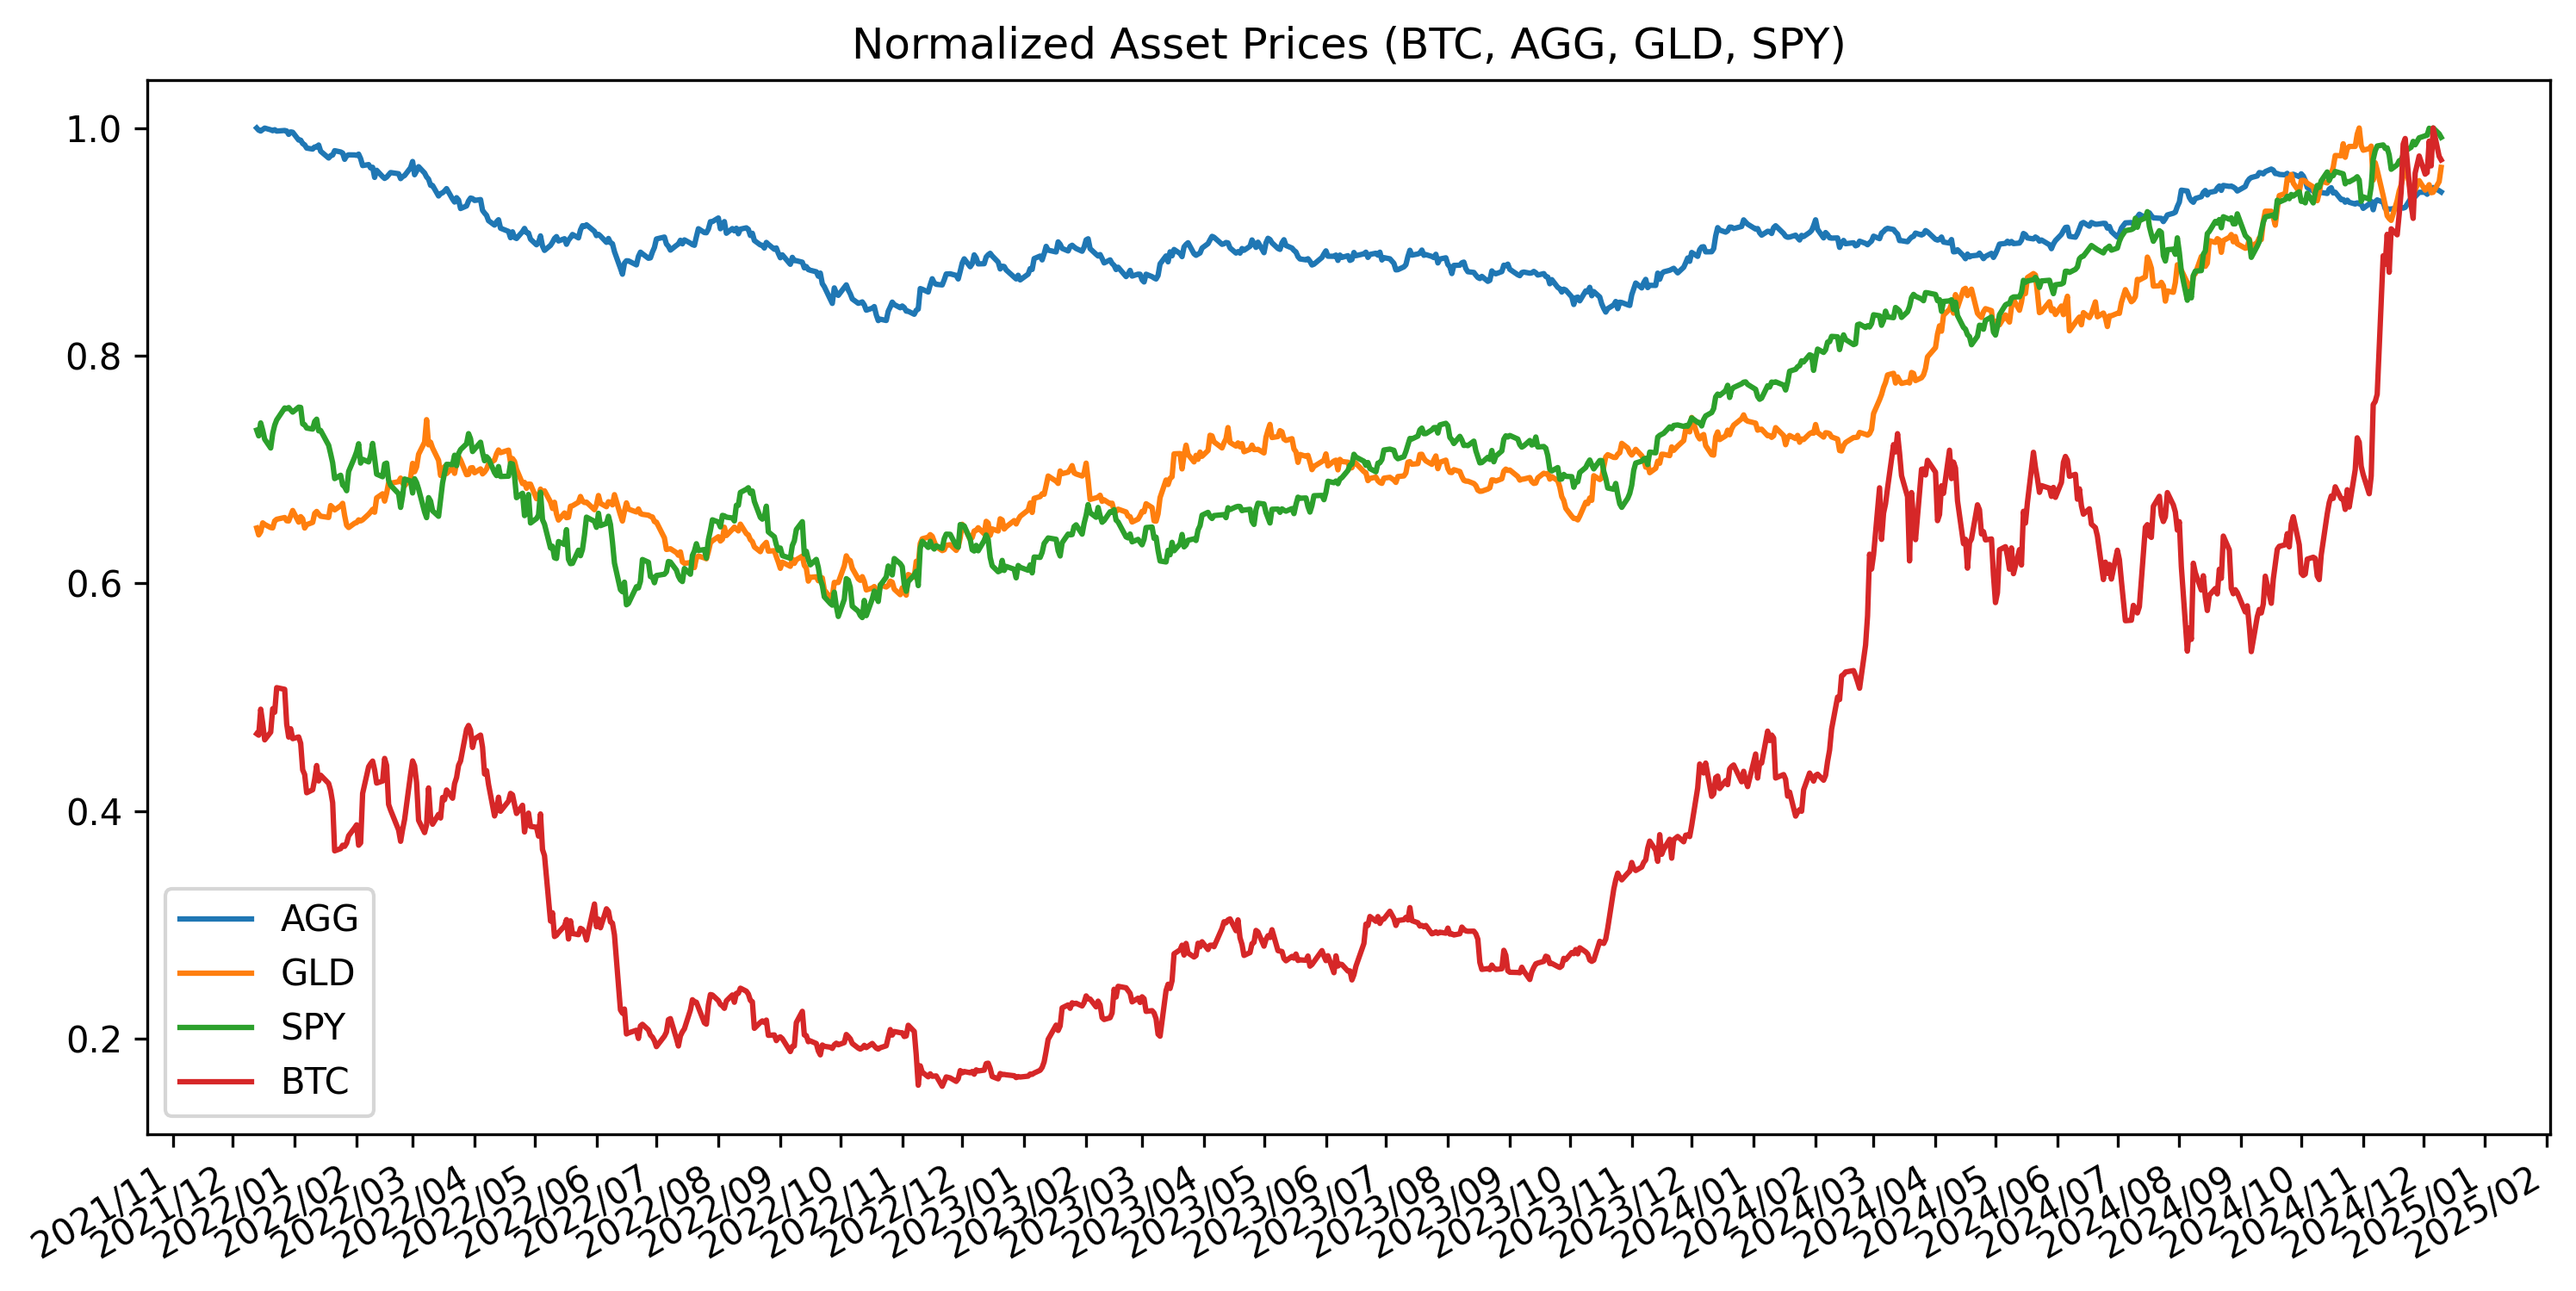
\includegraphics[width=\textwidth]{pre tex code/Figure/normalized_asset_prices.png}
             \end{center}
        \end{column}
        \end{columns}
    \end{frame}

    \begin{frame}{Correlation Anlysis}
        \begin{columns}
        \begin{column}{0.5\textwidth}
        \begin{itemize}
            \item<1-> The figure illustrates the rolling 30-day correlation between differnt asset class.
            \item<2-> Bitcoin shows a moderate positive correlation with the S\&P 500 Index, while its relationships with COMEX Gold Futures and Aggregate Oil Futures are weaker and more variable, reflecting differing macroeconomic influences and market-specific dynamics.
           
        \end{itemize}
        \end{column}
        \begin{column}{0.6\textwidth}  %%<--- here
            \begin{center}
             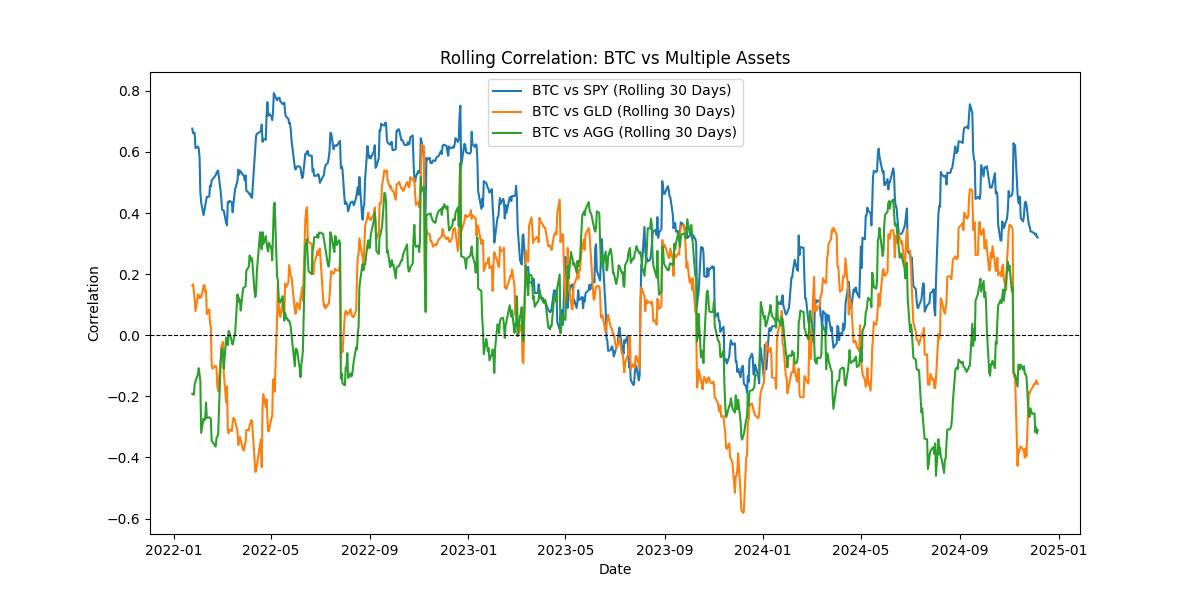
\includegraphics[width=\textwidth]{pre tex code/Figure/rolling_correlation_multi.png}
             \end{center}
        \end{column}
        \end{columns}
    \end{frame}

  \begin{frame}{Correlation Anlysis}
        \begin{columns}
        \begin{column}{0.5\textwidth}
        \begin{itemize}
            
            \item<1-> Correlation heatmap better visualizes the relationship
        \end{itemize}
        \end{column}
        \begin{column}{0.6\textwidth}  %%<--- here
            \begin{center}
             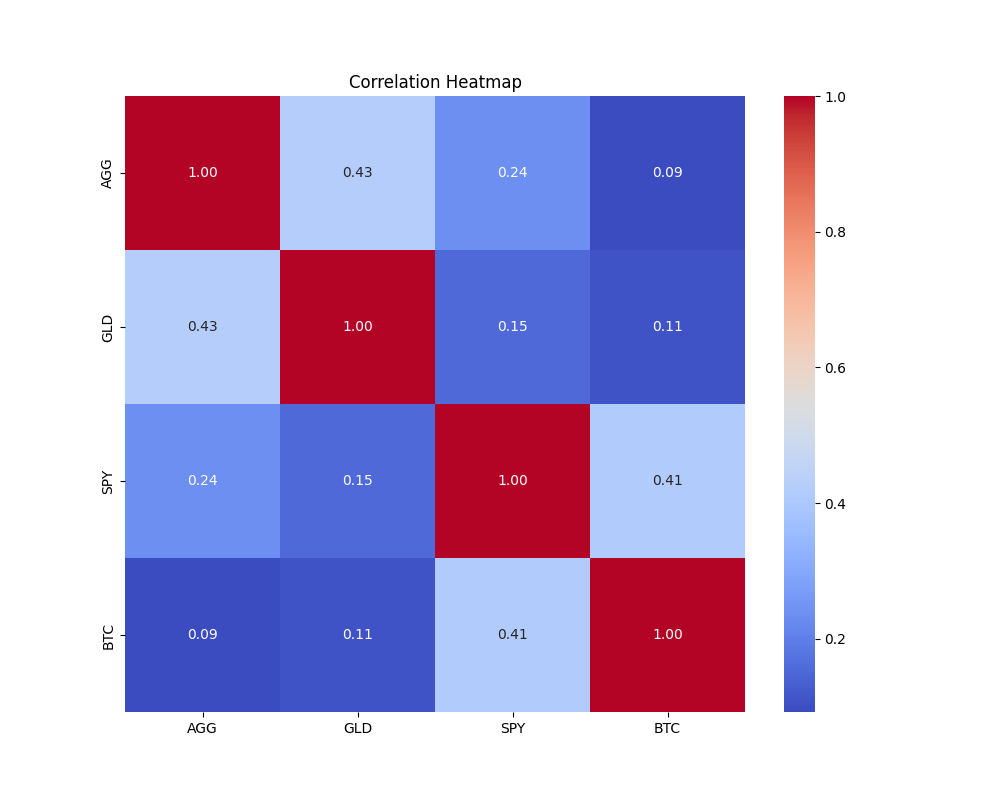
\includegraphics[width=\textwidth]{pre tex code/Figure/correlation_heatmap.png}
             \end{center}
        \end{column}
        \end{columns}
    \end{frame}

    \begin{frame}{Long Short-Term Memory Model}
        \begin{columns}
        \begin{column}{0.5\textwidth}
        \begin{itemize}
            \item<1-> The figure represents the heatmap of LSTM correlation matrix, revealing the relationships between the four financial assets.
            \item<2-> The matrix demonstrates an exceptionally high degree of correlation across all assets
            \item<3-> This matrix reveals different results from the other heatmap, the differences arise from their distinct methodologies....
        \end{itemize}
        \end{column}
        \begin{column}{0.5\textwidth}  %%<--- here
            \begin{center}
             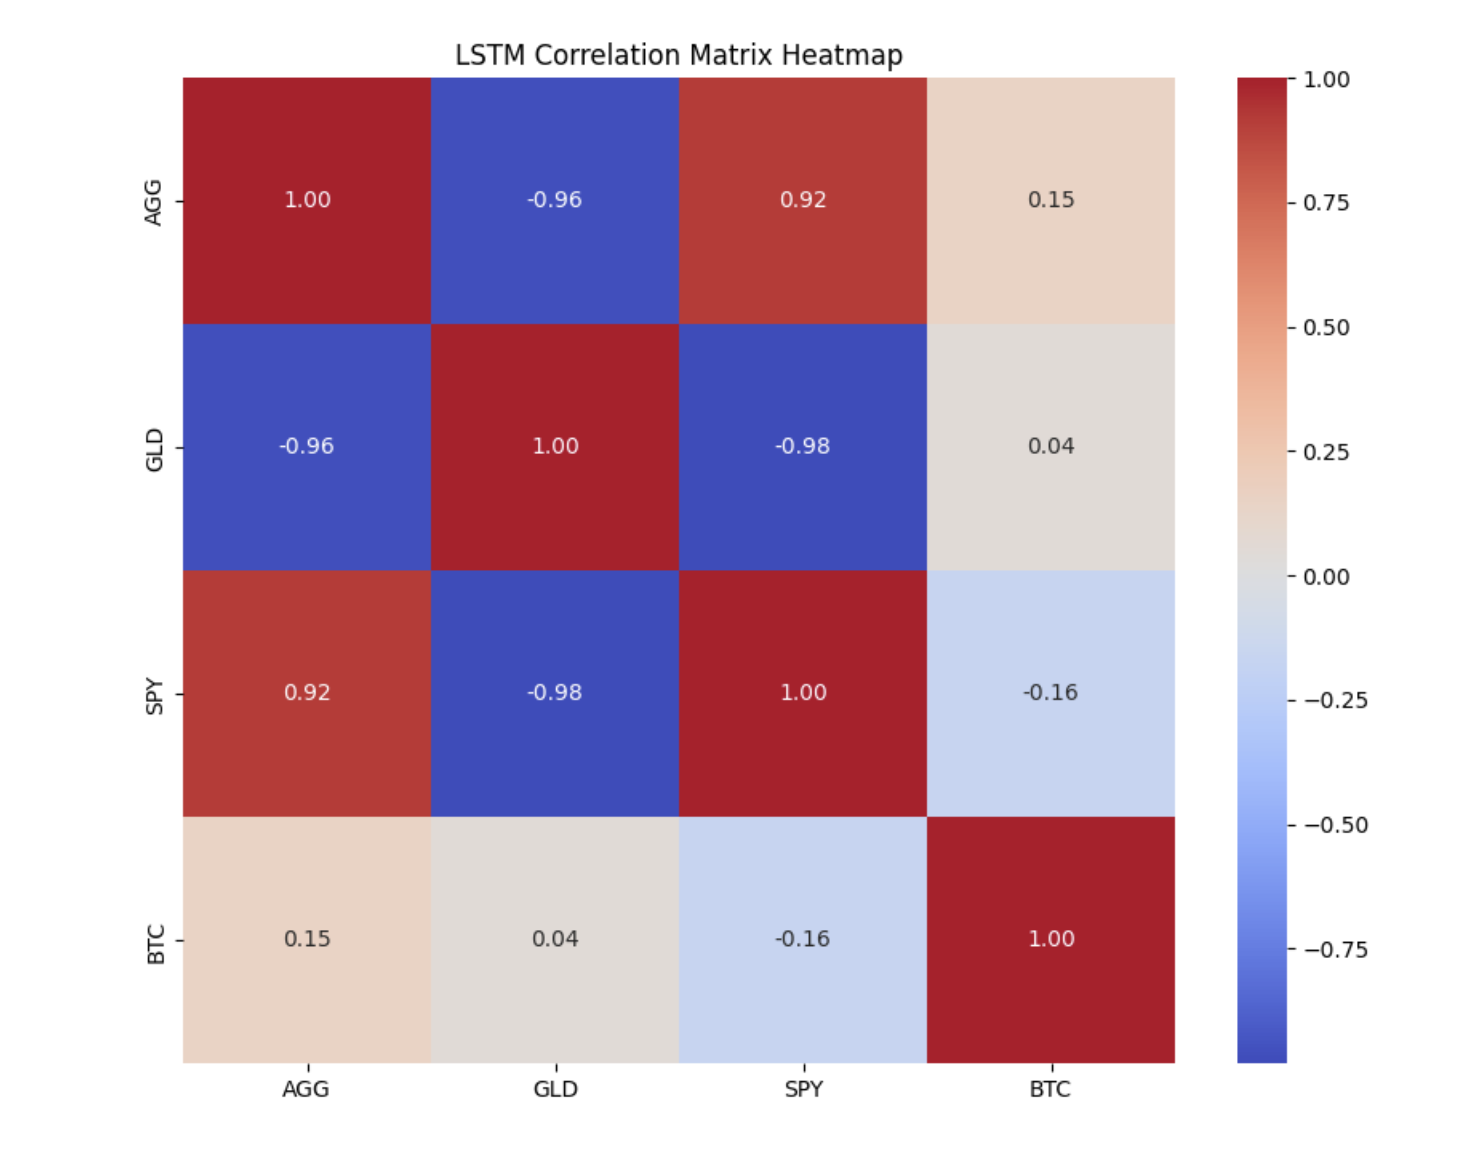
\includegraphics[width=\textwidth]{pre tex code/Figure/lstm_correlation_heatmap_with_labels.png}
             \end{center}
        \end{column}
        \end{columns}
    \end{frame}


  
    
    